\documentclass[12pt,letterpaper]{article}
\usepackage{pdfpages}
\usepackage{fancyhdr}
\usepackage[colorlinks=true, urlcolor=blue, linkcolor=blue]{hyperref}
\usepackage{graphicx}
\usepackage[top=1.4in, left=0.5in, right=0.5in, bottom=0.8in]{geometry}
\usepackage[T1]{fontenc}
\usepackage{helvet}
\pagestyle{fancy}
\renewcommand{\headrulewidth}{0pt}
\renewcommand{\footrulewidth}{0pt}
\setlength{\parindent}{0em}
\setlength{\parskip}{1em}


\fancyfoot[C]{\setlength{\unitlength}{1in}\begin{picture}(5,0)\put(-1.8,-1){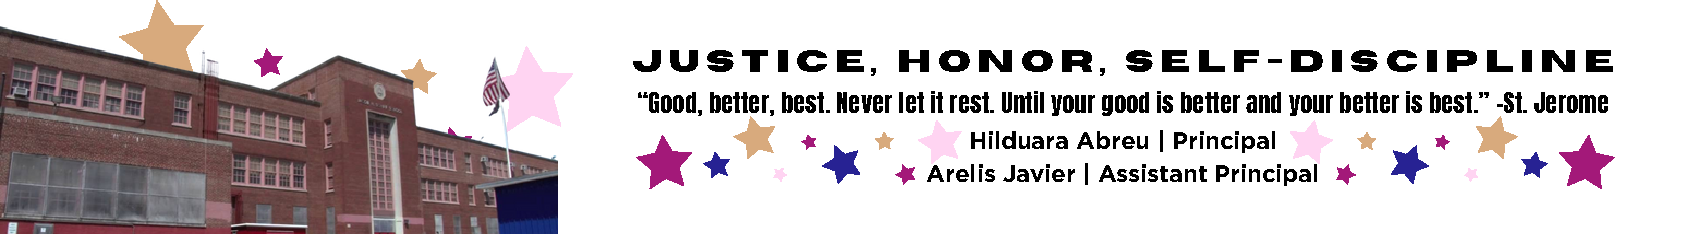
\includegraphics[width=8.8in,height=1.3in]{logo-1}}\end{picture}}
\fancyhead[C]{\setlength{\unitlength}{1in}\begin{picture}(5,0)\put(-1.9,-1){
\includegraphics[width=8.9in,height=1.3in]{logo-2}}\end{picture}}

\pagenumbering{gobble}
\addtolength{\evensidemargin}{-2in}
\addtolength{\topmargin}{-0.5in}
\addtolength{\textwidth}{0in}
%%%%%%%%%%%%%%%%%%%%%%%%%%%%%%%%%%%%%%%%%%%%%%%%%%%%%%%%%%%%%%%%%%

\begin{document}
\vspace*{0.5in}
Date: \href{https://www.ps192.org/apps/bbmessages/show_bbm.jsp?REC_ID=139439}{September 14, 2023} 

\textbf{Sujeto: Horario Escolar}

Un horario escolar especifica la hora de inicio y la duración de uno o más períodos de instrucción de cada día. Un horario diario consistente y rutinario
les ofrece a los niños una disciplina de trabajo durante la semana de clase. Un
horario escolar ayuda a los niños a:
\begin{itemize}
\item Sentirse en control de su entorno.
\item Sentirse seguro, protegido y cómodo.
\item Poder realizar una actividad o tarea.
\item Participar en el aprendizaje.
\end{itemize}
Al igual que los adultos, los niños se sienten más confiados y seguros cuando sus
actividades diarias son predecibles y familiares.

\begin{center}
	\LARGE
    \begin{tabular}{|c|c|c|c|}
    \hline
    \textbf{Periodo} & \textbf{Hora de inicio} & \textbf{Hora de finalización} & \textbf{Duración} \\  
    \hline
    1 & 08:00 AM & 08:45 AM & 45 minutos \\
    \hline
    2 & 08:45 AM & 09:30 AM & 45 minutos \\
    \hline
    3 & 09:30 AM & 10:15 AM & 45 minutos \\
    \hline
    4 & 10:15 AM & 11:05 AM & 50 minutos \\
    \hline
    5 & 11:05 AM & 11:55 PM & 50 minutos \\
    \hline
    6 & 11:55 PM & 12:40 PM & 45 minutos \\
    \hline
    7 & 12:40 PM & 01:30 PM & 50 minutos \\
    \hline
    8 & 01:30 PM & 02:15 PM & 45 minutos \\
    \hline
    \end{tabular}
    \end{center}



\end{document}
